\documentclass[conference]{IEEEtran}
\IEEEoverridecommandlockouts
\usepackage{cite}
\usepackage{amsmath,amssymb,amsfonts}
\usepackage{graphicx}
\usepackage{booktabs}
\usepackage{array}
\usepackage{algorithm}
\usepackage{algorithmic}
\usepackage{url}
\usepackage[hidelinks]{hyperref}

% Numerical results quoted in the text.
\newcommand{\BfourAcc}{59.25}
\newcommand{\BfourCS}{8.28}
\newcommand{\BfourFone}{56.87}
\newcommand{\BfourGap}{22.61}
\newcommand{\BfourIDAcc}{79.40}
\newcommand{\BfourIDFone}{79.47}
\newcommand{\BfourParams}{47{,}432}
\newcommand{\BfourSelVal}{67.18}
\newcommand{\BfourTrainAcc}{81.91}
\newcommand{\BfourVal}{67.18}
\newcommand{\BfourWorst}{25.81}
\newcommand{\BoneAcc}{60.38}
\newcommand{\BoneCS}{7.71}
\newcommand{\BoneFone}{58.73}
\newcommand{\BoneGap}{22.14}
\newcommand{\BoneIDAcc}{80.86}
\newcommand{\BoneIDFone}{80.87}
\newcommand{\BoneLatency}{2.82}
\newcommand{\BoneMinutes}{1.86}
\newcommand{\BoneOfiveAcc}{59.6}
\newcommand{\BoneOfiveCS}{4.00}
\newcommand{\BoneOfiveFone}{58.19}
\newcommand{\BoneOoneAcc}{58.6}
\newcommand{\BoneOoneCS}{9.94}
\newcommand{\BoneOoneFone}{55.73}
\newcommand{\BoneOthreeAcc}{63.0}
\newcommand{\BoneOthreeCS}{9.19}
\newcommand{\BoneOthreeFone}{62.27}
\newcommand{\BoneParams}{47{,}432}
\newcommand{\BoneSelVal}{69.05}
\newcommand{\BoneTrainAcc}{84.82}
\newcommand{\BoneVal}{69.05}
\newcommand{\BoneWorst}{35.67}
\newcommand{\BthreeAcc}{60.98}
\newcommand{\BthreeCS}{8.99}
\newcommand{\BthreeFone}{59.32}
\newcommand{\BthreeGap}{21.67}
\newcommand{\BthreeIDAcc}{80.99}
\newcommand{\BthreeIDFone}{80.99}
\newcommand{\BthreeOfiveAcc}{62.0}
\newcommand{\BthreeOfiveCS}{4.07}
\newcommand{\BthreeOfiveFone}{61.04}
\newcommand{\BthreeOoneAcc}{57.1}
\newcommand{\BthreeOoneCS}{11.12}
\newcommand{\BthreeOoneFone}{53.77}
\newcommand{\BthreeOthreeAcc}{63.9}
\newcommand{\BthreeOthreeCS}{11.78}
\newcommand{\BthreeOthreeFone}{63.16}
\newcommand{\BthreeParams}{47{,}432}
\newcommand{\BthreeSelVal}{68.35}
\newcommand{\BthreeTrainAcc}{85.16}
\newcommand{\BthreeVal}{68.35}
\newcommand{\BthreeWorst}{38.36}
\newcommand{\BtwoAcc}{62.59}
\newcommand{\BtwoCS}{9.54}
\newcommand{\BtwoFone}{60.53}
\newcommand{\BtwoGap}{23.37}
\newcommand{\BtwoIDAcc}{83.87}
\newcommand{\BtwoIDFone}{83.90}
\newcommand{\BtwoParams}{47{,}432}
\newcommand{\BtwoSelVal}{67.74}
\newcommand{\BtwoTrainAcc}{87.58}
\newcommand{\BtwoVal}{67.74}
\newcommand{\BtwoWorst}{35.83}
\newcommand{\CSRelReduction}{20.4}
\newcommand{\CfiveAcc}{60.42}
\newcommand{\CfiveCS}{7.14}
\newcommand{\CfiveClapFone}{81.10}
\newcommand{\CfiveFone}{58.62}
\newcommand{\CfiveGap}{22.20}
\newcommand{\CfiveIDAcc}{80.74}
\newcommand{\CfiveIDFone}{80.82}
\newcommand{\CfiveLatency}{4.08}
\newcommand{\CfiveMinutes}{2.97}
\newcommand{\CfiveOfiveAcc}{60.6}
\newcommand{\CfiveOfiveCS}{4.81}
\newcommand{\CfiveOfiveFone}{59.19}
\newcommand{\CfiveOoneAcc}{58.0}
\newcommand{\CfiveOoneCS}{9.12}
\newcommand{\CfiveOoneFone}{54.88}
\newcommand{\CfiveOoneSlideClap}{89}
\newcommand{\CfiveOoneSlideCorrect}{112}
\newcommand{\CfiveOoneSlideN}{675}
\newcommand{\CfiveOoneSlidePush}{186}
\newcommand{\CfiveOthreeAcc}{62.7}
\newcommand{\CfiveOthreeCS}{7.48}
\newcommand{\CfiveOthreeFone}{61.80}
\newcommand{\CfiveParams}{47{,}042}
\newcommand{\CfivePushFone}{61.42}
\newcommand{\CfiveSlideFone}{44.69}
\newcommand{\CfiveTrainAcc}{84.11}
\newcommand{\CfiveVal}{67.65}
\newcommand{\CfiveWorst}{34.14}
\newcommand{\CfiveZigzagFone}{42.46}
\newcommand{\CfourAcc}{60.57}
\newcommand{\CfourCS}{9.83}
\newcommand{\CfourFone}{58.57}
\newcommand{\CfourGap}{21.82}
\newcommand{\CfourIDAcc}{80.33}
\newcommand{\CfourIDFone}{80.38}
\newcommand{\CfourParams}{47{,}042}
\newcommand{\CfourTrainAcc}{84.23}
\newcommand{\CfourVal}{67.59}
\newcommand{\CfourWorst}{34.22}
\newcommand{\ConeAcc}{61.54}
\newcommand{\ConeCS}{8.97}
\newcommand{\ConeClapFone}{80.51}
\newcommand{\ConeFone}{59.35}
\newcommand{\ConeGap}{20.51}
\newcommand{\ConeIDAcc}{79.81}
\newcommand{\ConeIDFone}{79.85}
\newcommand{\ConeLatency}{2.93}
\newcommand{\ConeMinutes}{2.22}
\newcommand{\ConeOfiveAcc}{60.1}
\newcommand{\ConeOfiveCS}{3.85}
\newcommand{\ConeOfiveFone}{57.33}
\newcommand{\ConeOoneAcc}{60.2}
\newcommand{\ConeOoneCS}{14.38}
\newcommand{\ConeOoneFone}{56.96}
\newcommand{\ConeOoneSlideClap}{158}
\newcommand{\ConeOoneSlideCorrect}{113}
\newcommand{\ConeOoneSlideN}{675}
\newcommand{\ConeOoneSlidePush}{92}
\newcommand{\ConeOthreeAcc}{64.3}
\newcommand{\ConeOthreeCS}{8.67}
\newcommand{\ConeOthreeFone}{63.76}
\newcommand{\ConeParams}{47{,}042}
\newcommand{\ConePushFone}{65.72}
\newcommand{\ConeSlideFone}{47.92}
\newcommand{\ConeTrainAcc}{83.07}
\newcommand{\ConeVal}{67.25}
\newcommand{\ConeWorst}{31.81}
\newcommand{\ConeZigzagFone}{38.80}
\newcommand{\CthreeAcc}{60.73}
\newcommand{\CthreeCS}{9.09}
\newcommand{\CthreeFone}{58.63}
\newcommand{\CthreeGap}{20.52}
\newcommand{\CthreeIDAcc}{79.07}
\newcommand{\CthreeIDFone}{79.15}
\newcommand{\CthreeParams}{47{,}042}
\newcommand{\CthreeTrainAcc}{83.41}
\newcommand{\CthreeVal}{67.78}
\newcommand{\CthreeWorst}{33.18}
\newcommand{\CtwoAcc}{61.46}
\newcommand{\CtwoCS}{7.78}
\newcommand{\CtwoFone}{59.21}
\newcommand{\CtwoGap}{21.80}
\newcommand{\CtwoIDAcc}{80.95}
\newcommand{\CtwoIDFone}{81.01}
\newcommand{\CtwoParams}{47{,}042}
\newcommand{\CtwoTrainAcc}{83.90}
\newcommand{\CtwoVal}{68.00}
\newcommand{\CtwoWorst}{29.16}
\newcommand{\CzeroAcc}{59.16}
\newcommand{\CzeroCS}{9.34}
\newcommand{\CzeroFone}{56.41}
\newcommand{\CzeroGap}{16.63}
\newcommand{\CzeroIDAcc}{73.07}
\newcommand{\CzeroIDFone}{73.04}
\newcommand{\CzeroParams}{23{,}520}
\newcommand{\CzeroTrainAcc}{77.68}
\newcommand{\CzeroVal}{65.39}
\newcommand{\CzeroWorst}{22.48}
\newcommand{\DFiveBestAcc}{{+}0.03}
\newcommand{\DFiveBestAccHi}{{+}1.20}
\newcommand{\DFiveBestAccLo}{$-$1.30}
\newcommand{\DFiveBestCS}{$-$0.57}
\newcommand{\DFiveBestCSHi}{{+}0.54}
\newcommand{\DFiveBestCSLo}{$-$1.68}
\newcommand{\DFiveBestFone}{$-$0.11}
\newcommand{\DFiveBestFoneHi}{{+}1.16}
\newcommand{\DFiveBestFoneLo}{$-$1.40}
\newcommand{\DFiveFourAcc}{$-$0.16}
\newcommand{\DFiveFourAccHi}{{+}0.59}
\newcommand{\DFiveFourAccLo}{$-$0.89}
\newcommand{\DFiveFourCS}{$-$2.69}
\newcommand{\DFiveFourCSHi}{$-$1.21}
\newcommand{\DFiveFourCSLo}{$-$4.25}
\newcommand{\DFiveFourFone}{{+}0.05}
\newcommand{\DFiveFourFoneHi}{{+}0.95}
\newcommand{\DFiveFourFoneLo}{$-$0.81}
\newcommand{\DFiveOneAcc}{$-$1.13}
\newcommand{\DFiveOneAccHi}{{+}0.06}
\newcommand{\DFiveOneAccLo}{$-$2.31}
\newcommand{\DFiveOneCS}{$-$1.83}
\newcommand{\DFiveOneCSHi}{$-$0.39}
\newcommand{\DFiveOneCSLo}{$-$3.66}
\newcommand{\DFiveOneFone}{$-$0.73}
\newcommand{\DFiveOneFoneHi}{{+}0.51}
\newcommand{\DFiveOneFoneLo}{$-$2.20}
\newcommand{\DFiveThreeAcc}{$-$0.31}
\newcommand{\DFiveThreeAccHi}{{+}0.54}
\newcommand{\DFiveThreeAccLo}{$-$1.31}
\newcommand{\DFiveThreeCS}{$-$1.95}
\newcommand{\DFiveThreeCSHi}{$-$0.62}
\newcommand{\DFiveThreeCSLo}{$-$3.38}
\newcommand{\DFiveThreeFone}{$-$0.00}
\newcommand{\DFiveThreeFoneHi}{{+}0.91}
\newcommand{\DFiveThreeFoneLo}{$-$1.12}
\newcommand{\DFiveTwoAcc}{$-$1.05}
\newcommand{\DFiveTwoAccHi}{$-$0.21}
\newcommand{\DFiveTwoAccLo}{$-$2.07}
\newcommand{\DFiveTwoCS}{$-$0.64}
\newcommand{\DFiveTwoCSHi}{{+}0.27}
\newcommand{\DFiveTwoCSLo}{$-$1.60}
\newcommand{\DFiveTwoFone}{$-$0.59}
\newcommand{\DFiveTwoFoneHi}{{+}0.52}
\newcommand{\DFiveTwoFoneLo}{$-$2.05}
\newcommand{\DOneZeroAcc}{{+}2.39}
\newcommand{\DOneZeroAccHi}{{+}3.46}
\newcommand{\DOneZeroAccLo}{{+}1.33}
\newcommand{\DOneZeroCS}{$-$0.37}
\newcommand{\DOneZeroCSHi}{{+}1.73}
\newcommand{\DOneZeroCSLo}{$-$2.59}
\newcommand{\DOneZeroFone}{{+}2.94}
\newcommand{\DOneZeroFoneHi}{{+}3.92}
\newcommand{\DOneZeroFoneLo}{{+}2.04}
\newcommand{\DiffGesFiOneCO}{$-$26.24}
\newcommand{\DiffGesFiOneID}{$-$16.55}
\newcommand{\DiffWiZeAblID}{$-$7.65}
\newcommand{\DiffWiZeOneCO}{$-$36.15}
\newcommand{\FeatMs}{214}
\newcommand{\GateDiffRatio}{68.0}
\newcommand{\GateDopLockedRatio}{65.6}
\newcommand{\GateDopOrigAnt}{23.7}
\newcommand{\GateDopOrigRatio}{52.4}
\newcommand{\GateEpochs}{45}
\newcommand{\GateLocked}{80.9}
\newcommand{\GateLockedTrain}{86.3}
\newcommand{\GateNfits}{22}
\newcommand{\GateNheld}{540}
\newcommand{\GateNtrain}{2159}
\newcommand{\GateOrig}{38.9}
\newcommand{\GateOrigTrain}{47.4}
\newcommand{\GateUnwrapAnt}{24.4}
\newcommand{\GateUnwrapRatio}{46.7}
\newcommand{\LamHighCS}{6.97}
\newcommand{\LamHighFone}{57.19}
\newcommand{\LamLowCS}{6.52}
\newcommand{\LamLowFone}{59.89}
\newcommand{\LamMidCS}{8.89}
\newcommand{\LamMidFone}{57.44}
\newcommand{\NBoot}{1{,}000}
\newcommand{\NExcluded}{3}
\newcommand{\NIDTest}{810}
\newcommand{\NRuns}{96}
\newcommand{\NTarget}{1{,}349}
\newcommand{\NTrain}{3238}
\newcommand{\NTrainMax}{3239}
\newcommand{\NTrials}{6{,}750}
\newcommand{\NVal}{1{,}349}
\newcommand{\NValid}{6{,}747}
\newcommand{\RelGesFiOneCO}{$-$30.3}
\newcommand{\RelWiZeOneCO}{$-$37.4}
\newcommand{\RepGLSDABaseCO}{89.92}
\newcommand{\RepGLSDACO}{92.80}
\newcommand{\RepGesFiOneCO}{86.66}
\newcommand{\RepGesFiOneID}{97.29}
\newcommand{\RepGesFiOneOri}{66.35}
\newcommand{\RepGesFiSixCO}{96.45}
\newcommand{\RepGesFiThreeOri}{92.60}
\newcommand{\RepGesFiTwoOri}{82.46}
\newcommand{\RepKooCD}{56.61}
\newcommand{\RepKooCU}{54.43}
\newcommand{\RepKooID}{99.31}
\newcommand{\RepWiSROneCO}{88.80}
\newcommand{\RepWiZeAblCRU}{76.67}
\newcommand{\RepWiZeAblID}{88.39}
\newcommand{\RepWiZeOneCO}{96.57}
\newcommand{\RepWiZeOneID}{98.32}
\newcommand{\ShaShort}{0025f7d831f2}
\newcommand{\TorchVersion}{2.14.1{+}cu130}
\newcommand{\TrainHours}{3.62}


\newcommand{\Lcons}{\mathcal{L}_{\mathrm{cons}}}
\newcommand{\Lce}{\mathcal{L}_{\mathrm{CE}}}

\begin{document}

\title{Class-Consistent Prototype Learning for Single-Link Cross-Orientation WiFi Gesture Recognition: A Strict Domain-Generalization Study}

\author{
\IEEEauthorblockN{Muhammad Huzaifa Khalid}
\IEEEauthorblockA{\textit{FAST School of Computing}\\
\textit{National University of Computer and Emerging Sciences}\\
Islamabad, Pakistan\\
i232508@isb.nu.edu.pk}
\and
\IEEEauthorblockN{Abdullah Asim}
\IEEEauthorblockA{\textit{FAST School of Computing}\\
\textit{National University of Computer and Emerging Sciences}\\
Islamabad, Pakistan\\
i232621@isb.nu.edu.pk}
}

\maketitle

\begin{abstract}
Device-free gesture recognition from WiFi channel state information (CSI) loses accuracy when the user faces a direction that was not seen in training, and most systems that cope with this shift fuse several receivers or adapt on target-domain data. This paper studies the setting that remains when neither is available: one transmitter, one receiver and no target calibration. The proposed model fuses a CSI-ratio phase map and a Doppler map from the same link in a \CfiveParams-parameter network, classifies with source-built cosine prototypes, and is trained with a class-consistency loss and a query augmentation curriculum. It is evaluated on Widar3.0 Room~1 (nine users, six gestures, \NValid{} trials) in three leave-one-orientation-out tasks with three seeds, against five ablation arms and four domain-generalization baselines (ERM, Deep CORAL, DANN, Mixup), 96 trainings in total. A preprocessing study shows that applying the Hampel filter to the CSI ratio and using phase-derivative and band-passed Doppler maps raises held-out accuracy on non-target orientations from \GateOrig\% to \GateLocked\%. On unseen orientations the proposed method reaches \CfiveAcc\% accuracy and lowers the clap/slide pair error from \ConeCS\% to \CfiveCS\% (\DFiveOneCS{} points, 95\% interval \DFiveOneCSLo{} to \DFiveOneCSHi), an effect traced to the augmentation curriculum. Accuracy and macro-F1 do not improve over the matched baseline (\DFiveOneAcc{} and \DFiveOneFone{} points, intervals containing zero), and all domain-generalization methods stay within about two points of ERM. The roughly 20-point gap between in-domain and unseen-orientation accuracy is the main limitation of strictly single-link sensing in this setting.
\end{abstract}

\begin{IEEEkeywords}
WiFi sensing, channel state information, gesture recognition, domain generalization, single link, prototype learning
\end{IEEEkeywords}

\section{Introduction}
WiFi channel state information (CSI) describes how each subcarrier of a link is attenuated and phase-shifted along its propagation paths. A moving hand changes some of these paths, so CSI recorded by commodity network cards can be used to recognise gestures without cameras or worn devices \cite{halperin2011csitool,zhang2022widar3}. The difficulty is that the same gesture produces different CSI when the user stands elsewhere, faces another direction or is a different person. A model trained under one set of conditions, or domain, then performs worse in another \cite{zhang2022widar3,zhou2023dgsurvey}.

Published systems reduce this domain shift in three main ways. Multi-receiver systems combine several links into features that depend less on the user's position, such as the body-coordinate velocity profile of Widar3.0 \cite{zhang2022widar3} or the multi-view CSI-ratio and Doppler templates of UniFi \cite{liu2023unifi}. Adaptation methods use labelled or unlabelled data from the target domain \cite{feng2022wilearner,yan2025wisfdagr,jiao2025mswiar}. Domain-generalization methods train only on source domains and use adversarial alignment, style randomisation or data mixing to obtain features that transfer \cite{jiang2018ei,liu2023wisr,zhang2026gesfi}. In many deployments only one access point and one client are under the operator's control, and no calibration data can be collected from new users. That leaves the single-link, zero-calibration case, which has received less attention: WiZeCSi reports that its single-link accuracy depends on training with data from six receivers \cite{dai2026wizecsi}, and a recent single-link finger-sensing system reaches about 55\% across users and days despite 99\% in-domain accuracy \cite{koo2026dualaxis}.

A second gap concerns similar gestures. Clap and slide are both short horizontal hand movements, and WiZeCSi reports slide as its least accurate gesture, confused with sweep and clap \cite{dai2026wizecsi}. Aggregate accuracy can hide such pairwise errors, and existing work rarely reports them.

This paper asks whether source-trained class-consistency learning, combined with same-link phase/Doppler fusion and an augmentation curriculum, reduces confusion between similar gestures and improves single-link cross-orientation accuracy without target calibration. Its contributions are as follows.
\begin{itemize}
\item A strict single-link protocol on Widar3.0 Room~1: one receiver and one CSI ratio, three leave-one-orientation-out tasks with a separate source-validation orientation, fixed trial-level splits, three seeds and a paired participant-level bootstrap.
\item A preprocessing study with \GateNfits{} controlled fits on orientations that are never targets. It shows that the position of the Hampel filter and the definition of the phase and Doppler maps decide whether a single-link model learns the gestures at all (\GateOrig\% versus \GateLocked\% held-out accuracy).
\item A compact class-consistent prototype model (C5) with a controlled ablation (C0--C4) and four domain-generalization baselines on the same encoder. C5 lowers the clap/slide pair error by \CSRelReduction\% relative to its matched baseline, an effect traced to the augmentation curriculum, while its accuracy and macro-F1 do not improve.
\item A comparison with three base papers on single-link and cross-domain WiFi gesture recognition that separates differences of protocol from differences of method.
\end{itemize}
Section~\ref{sec:related} reviews related work, Section~\ref{sec:method} describes the method and Section~\ref{sec:setup} the experimental setup. Results, the base-paper comparison and the ablation follow in Sections~\ref{sec:results}--\ref{sec:ablation}. Section~\ref{sec:discussion} discusses limitations and Section~\ref{sec:conclusion} concludes.

\section{Related Work}\label{sec:related}
\subsection{Multi-link and model-based features}
Widar3.0 derives a body-coordinate velocity profile from the Doppler shifts seen by several receivers, which makes the feature largely independent of location and orientation, but it needs at least three links \cite{zhang2022widar3}. WiGRUNT applies dual attention to CSI-ratio maps of six links \cite{gu2022wigrunt}, UniFi combines CSI-ratio and Doppler templates in a multi-view network that needs at least two antenna pairs \cite{liu2023unifi}, and WiDual uses spatial and channel attention on CSI ratios from two to six links \cite{cao2025widual}. These systems reach over 90\% across orientations, but their accuracy comes partly from the spatial diversity of several receivers. The CSI ratio itself, the quotient of two antennas on the same card, cancels the random phase offsets of commodity hardware and is the input most recent systems share \cite{zeng2019farsense}.

\subsection{Adaptation with target data}
Few-shot and adaptation methods reduce the gap with target-domain samples. Wi-Learner learns from one labelled target example per class \cite{feng2022wilearner}, WiGR uses modified prototypical networks with target data \cite{zhang2022wigr}, MSWiAR performs multi-source adaptation for single-transceiver scenarios \cite{jiao2025mswiar}, and Wi-SFDAGR adapts a source model on unlabelled target data \cite{yan2025wisfdagr}. All of them require data collection in the deployment domain, which this study excludes.

\subsection{Domain generalization}
EI aligns features adversarially using domain labels \cite{jiang2018ei}, and WiSR randomises signal style to generalise from source domains \cite{liu2023wisr}. GLSDA distils semantic knowledge from a large model to align gesture features \cite{cui2025glsda}. GesFi argues that physical labels such as orientation are a poor definition of domains for adversarial alignment and instead mines latent domains from the data \cite{zhang2026gesfi}. In computer vision, careful ERM training is a strong baseline that many generalization methods do not beat \cite{gulrajani2021lost}. The method studied here differs from these works in using class prototypes built from source orientations with an explicit per-class consistency term, rather than a domain discriminator, and in being evaluated on one receiver only.

\subsection{Single-link sensing}
WiZeCSi trains one network on CSI-ratio samples from all six receivers and all antenna pairs and tests on any single link, reaching 96.57\% across orientations; without its multi-ratio augmentation and link mixing, single-link in-domain accuracy falls to 88.39\% \cite{dai2026wizecsi}. Koo and Park use one ESP8266 link with a dual-axis Transformer and a graph network over segments from different domains, and report 54.43\% across users \cite{koo2026dualaxis}. Table~\ref{tab:related} summarises the studies most relevant to this paper.

\begin{table*}[t]
\centering
\caption{Summary of related studies. Accuracies are as reported by the authors under their own protocols (CO: cross-orientation).}
\label{tab:related}
\footnotesize
\setlength{\tabcolsep}{3pt}
\begin{tabular}{@{}p{2.3cm}p{2.3cm}p{2.9cm}p{1.9cm}p{1.7cm}p{5.0cm}@{}}
\toprule
Study & Links & Input & Target data & CO acc. (\%) & Main limitation for the single-link, zero-calibration case \\
\midrule
Widar3.0 \cite{zhang2022widar3} & 6 receivers & body-coordinate velocity profile & none & 82.6--92.4$^{a}$ & needs at least three links and the user's position \\
WiGRUNT \cite{gu2022wigrunt} & 6 & CSI ratio & none & -- & multi-link input \\
UniFi \cite{liu2023unifi} & 2--6 & CSI ratio + Doppler & none & -- & needs at least two antenna pairs \\
WiSR \cite{liu2023wisr} & 1 pair & CSI & none & 88.80$^{b}$ & evaluated with four training orientations \\
GLSDA \cite{cui2025glsda} & 1 location & CSI-ratio branch & none & 92.80 & large-model teacher, different split \\
Wi-SFDAGR \cite{yan2025wisfdagr} & multi-device & CSI-ratio phase & unlabelled & 97.17 & adapts on target data \\
GesFi \cite{zhang2026gesfi} & 1 or 6 pairs & CSI-ratio phase + Doppler & none & 86.66 (1 pair) & pretrained ResNet18, four training orientations \\
WiZeCSi \cite{dai2026wizecsi} & 6 in training, 1 at test & CSI-ratio amplitude + phase & none & 96.57 & needs six receivers during training \\
Koo and Park \cite{koo2026dualaxis} & 1 & CSI amplitude & none & n/a & 54.43\% cross-user; different task \\
This work & 1 & CSI-ratio phase + Doppler & none & \CfiveAcc & three training orientations, see Section~\ref{sec:discussion} \\
\bottomrule
\end{tabular}\\[2pt]
\raggedright\footnotesize $^{a}$Cross-domain range reported for six receivers. $^{b}$Single-pair result as reported in \cite{zhang2026gesfi}.
\end{table*}

\section{Proposed Methodology}\label{sec:method}
\subsection{Problem formulation}
Let $\mathcal{O}=\{1,\dots,5\}$ be the face orientations of the user and $\mathcal{Y}=\{1,\dots,C\}$ the $C=6$ gestures. A trial $\mathbf{x}$ is the CSI recorded by antennas 1 and 2 of one receiver during one gesture. For a task, the training orientations $\mathcal{O}_s\subset\mathcal{O}$ ($|\mathcal{O}_s|=3$), a validation orientation $o_v$ and a target orientation $o_t$ are disjoint. A model $f$ is trained on labelled trials from $\mathcal{O}_s$ only, its checkpoint is chosen on $o_v$, and it is evaluated once on $o_t$. No target trial, label or statistic is used before the evaluation. Figure~\ref{fig:arch} shows the pipeline.

\begin{figure*}[t]
\centering
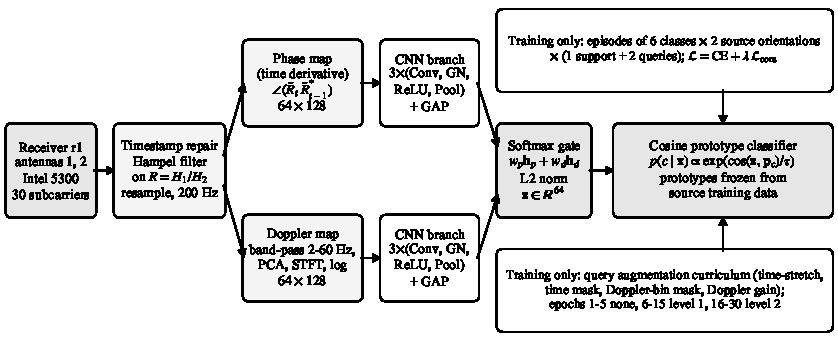
\includegraphics[width=0.95\textwidth]{figures/architecture.pdf}
\caption{Pipeline of the proposed method. Two maps are computed from the CSI ratio of one receiver, encoded by two small CNN branches and fused by a learned gate. Classification uses cosine similarity to class prototypes built from source training data. The boxes marked ``training only'' are not used at test time.}
\label{fig:arch}
\end{figure*}

\subsection{CSI ratio and preprocessing}
For subcarrier $k$ and packet time $t$, the CSI ratio of the two antennas is
\begin{equation}
R_k(t)=\frac{H_{1,k}(t)}{H_{2,k}(t)+\epsilon},
\end{equation}
where $H_{a,k}(t)$ is the complex CSI of antenna $a$ and $\epsilon$ is $10^{-6}$ times the median of $|H_{2,k}|$. The common phase offsets of the card cancel in the ratio \cite{zeng2019farsense}. Packets are sorted by their 32-bit microsecond timestamps after unwrapping counter overflow, duplicates are removed, and a Hampel filter (window 7, threshold three scaled median absolute deviations) \cite{pearson2016hampel} is applied to the real and imaginary parts of $R_k(t)$. The ratio is linearly interpolated onto a 1\,kHz grid and resampled to 200\,Hz with a polyphase anti-aliasing filter. Trials shorter than 0.5\,s or with a packet gap over 100\,ms are excluded.

\textit{Phase map.} With $\tilde R_k(t)$ the ratio after a zero-phase 60\,Hz low-pass filter, the phase map is the phase change between consecutive samples,
\begin{equation}
\phi_k(t)=\angle\!\left(\tilde R_k(t)\,\tilde R_k^{*}(t-1)\right),
\end{equation}
which needs no phase unwrapping. The $30\times T$ map is resized to $64\times128$.

\textit{Doppler map.} The ratio is band-pass filtered between 2 and 60\,Hz (fourth-order zero-phase Butterworth), which removes the static and slowly drifting components. The centred subcarrier signals are projected on their first complex principal component $\mathbf{v}_1$, giving $s(t)=\mathbf{v}_1^{H}\bar{\mathbf{R}}(t)$. The map is $D(f,t)=\log\bigl(1+|\mathrm{STFT}\{s\}(f,t)|^2\bigr)$ for $|f|\le60$\,Hz, with a 64-sample Hann window, hop 16 and a 256-point FFT, resized to $64\times128$.

These two definitions were chosen by the preprocessing study of Section~\ref{sec:gate}, which compares them with the unwrapped phase and mean-removed Doppler maps used in earlier designs, using only orientations that are never targets.

\subsection{Encoder and prototype classifier}
Each map is processed by a branch of three blocks (3$\times$3 convolution with 16, 32 and 64 channels, GroupNorm with eight groups \cite{wu2018groupnorm}, ReLU, $2\times2$ max-pooling) and global average pooling, giving $\mathbf{h}_p,\mathbf{h}_d\in\mathbb{R}^{64}$. A two-weight gate fuses them:
\begin{equation}
\mathbf{z}=\frac{w_p\mathbf{h}_p+w_d\mathbf{h}_d}{\lVert w_p\mathbf{h}_p+w_d\mathbf{h}_d\rVert_2},\qquad (w_p,w_d)=\mathrm{softmax}(\mathbf{a}),
\end{equation}
with learnable $\mathbf{a}\in\mathbb{R}^2$. The model has \CfiveParams{} trainable parameters. Following prototypical networks \cite{snell2017protonet}, the class probability is
\begin{equation}
p(y=c\mid\mathbf{x})=\frac{\exp\bigl(\mathbf{z}^{\top}\mathbf{p}_c/\tau\bigr)}{\sum_{c'}\exp\bigl(\mathbf{z}^{\top}\mathbf{p}_{c'}/\tau\bigr)},
\end{equation}
with temperature $\tau=0.1$ and unit-norm prototypes $\mathbf{p}_c$. Each prototype gives the source orientations equal weight:
\begin{equation}
\mathbf{p}_c=\mathrm{n}\Bigl(\frac{1}{|\mathcal{O}_s|}\sum_{o\in\mathcal{O}_s}\mathrm{n}\bigl(\bar{\mathbf{z}}_{c,o}\bigr)\Bigr),
\end{equation}
where $\bar{\mathbf{z}}_{c,o}$ is the mean embedding of the training trials of class $c$ and orientation $o$, and $\mathrm{n}(\cdot)$ divides by the L2 norm. After training, the prototype bank is computed once from clean source embeddings and frozen.

\subsection{Episodic training and class consistency}
Each episode samples two of the three source orientations and, for every class and sampled orientation, one support and two query trials. Episode prototypes are built from the supports in the same equal-weight way. For class $c$ and orientation $o$ in an episode, let $\mathbf{m}_{c,o}$ be the normalised mean of its support and query embeddings and $\mathbf{m}_c=\mathrm{n}(\frac{1}{2}\sum_o\mathbf{m}_{c,o})$. The class-consistency loss is
\begin{equation}
\Lcons=\frac{1}{2C}\sum_{c=1}^{C}\sum_{o}\bigl(1-\mathbf{m}_{c,o}^{\top}\mathbf{m}_c\bigr),
\end{equation}
which is zero when every orientation places a class at the same point. It is computed on clean embeddings. The objective is
\begin{equation}
\mathcal{L}=\tfrac{1}{2}\bigl(\Lce(\mathbf{Q})+\Lce(\mathcal{A}(\mathbf{Q}))\bigr)+\lambda\Lcons,
\end{equation}
where $\Lce$ is the query cross-entropy, $\mathbf{Q}$ the clean queries, $\mathcal{A}$ the augmentation and $\lambda=0.1$. Without augmentation only the clean term is used. Supports are never augmented.

\textit{Augmentation curriculum.} $\mathcal{A}$ applies four label-preserving transforms to queries: a time stretch by a factor from $U(1-s,1+s)$, a time mask of up to $m$ frames, a mask of up to $f$ Doppler bins (Doppler map only), and a gain of up to $\pm g$\,dB applied to Doppler power before normalisation. Epochs 1--5 use no augmentation, epochs 6--15 use $(s,m,f,g)=(0.05,8,4,1)$ and epochs 16--30 use $(0.10,16,8,2)$. Algorithm~\ref{alg:train} summarises one training run.

\begin{algorithm}[t]
\caption{Training of the proposed model (C5)}
\label{alg:train}
\begin{algorithmic}[1]
\REQUIRE source trials of $\mathcal{O}_s$, validation trials of $o_v$, epochs $E=30$, $\lambda$
\FOR{$e=1$ \TO $E$}
\STATE set augmentation level from the curriculum for epoch $e$
\FOR{each of $\lceil N_{\mathrm{train}}/36\rceil$ episodes}
\STATE sample two orientations; one support and two queries per class and orientation
\STATE build episode prototypes from clean supports
\STATE $\mathcal{L}\leftarrow$ query cross-entropy (clean and augmented) $+\lambda\Lcons$
\STATE update parameters with AdamW
\ENDFOR
\STATE rebuild prototype bank from clean source embeddings
\STATE keep the checkpoint if validation macro-F1 on $o_v$ improves
\ENDFOR
\RETURN selected encoder and its frozen prototype bank
\end{algorithmic}
\end{algorithm}

\subsection{Controlled variants}
Five variants isolate the components. C0 uses the phase branch only. C1, the matched baseline, fuses both maps without consistency or augmentation. C2 adds the curriculum to C1, C3 adds the consistency loss to C1, and C4 combines consistency with a fixed augmentation level of $(0.08,13,6,1.6)$, the epoch-weighted mean of the curriculum, after the same warm-up. C5 is the full method. All variants share data, sampler, classifier, optimiser and seeds.

\section{Experimental Setup}\label{sec:setup}
\subsection{Dataset}
Widar3.0 \cite{zhang2022widar3} was recorded with Intel 5300 cards (one transmit and three receive antennas, 30 subcarrier groups, about 1,000 packets/s at 5.825\,GHz) \cite{halperin2011csitool}. This study uses session 20181130 (Room~1, a classroom), receiver r1 only and gestures 1--6: push\&pull, sweep, clap, slide, draw-O and draw-zigzag. The nine users (5, 10--17) performed every gesture five times at five locations and five orientations, giving \NTrials{} trials. Of these, \NExcluded{} were excluded for lasting under 0.5\,s, leaving \NValid. The other five receivers, gestures 7--9 and the dataset's velocity-profile and Doppler files, which fuse six receivers, are not used. Archive integrity was checked by SHA-256 and per-file CRC.

\subsection{Splits}
The three tasks are O1 (train on orientations 3, 4, 5, validate on 2, test on 1), O3 (train 1, 2, 5, validate 4, test 3) and O5 (train 2, 3, 4, validate 1, test 5). In each task, 20\% of the trials of every gesture and training orientation form a fixed in-domain test set, leaving \NTrain--\NTrainMax{} training trials, \NIDTest{} in-domain test trials and about \NVal{} validation and \NTarget{} target trials. Splits are made once at trial level and checked by assertions for disjointness and for the absence of the target orientation from all other partitions. Clipping limits (0.5th and 99.5th percentiles) and z-score statistics are computed per channel on the training partition only.

\subsection{Preprocessing study}\label{sec:gate}
Before any domain-generalization run, each candidate preprocessing was scored by a plain ERM classifier (the branch encoder with a linear head) on orientations 2 and 4 only, which are never targets: \GateNtrain{} training and \GateNheld{} held-out trials from a random split stratified by user, gesture and orientation. Two Hampel placements (on the raw antennas or on the ratio), four phase maps and six Doppler maps were compared. The chosen pipeline was required to exceed 70\% held-out accuracy with the fused model before the main experiments.

\subsection{Baselines}
Four domain-generalization baselines use the same fused encoder with a linear head on $\mathbf{z}/\tau$, balanced batches of 64 trials over gesture and orientation, and the same optimiser, epochs and checkpoint selection: B1 ERM; B2 Deep CORAL \cite{sun2016coral}, aligning the covariances of the three training orientations; B3 DANN \cite{ganin2015dann} with a two-layer orientation discriminator behind a gradient-reversal layer; and B4 Mixup \cite{zhang2018mixup} with $\alpha=0.2$. For B2, the unweighted CORAL term was about $10^{-3}$ of the cross-entropy on source data, so its weight was set to 1,000, following the original authors' guidance that the two losses be of similar size. The best external baseline is chosen by mean source-validation macro-F1, never by target results.

\subsection{Metrics and statistics}
The metrics are accuracy, macro-F1, worst-class F1 and the clap/slide pair error
\begin{equation}
E_{\mathrm{cs}}=\tfrac{1}{2}\bigl(P(\hat y=\text{slide}\mid y=\text{clap})+P(\hat y=\text{clap}\mid y=\text{slide})\bigr).
\end{equation}
The generalization gap is in-domain minus target macro-F1. Results are the mean and sample standard deviation over seeds 42, 43 and 44; the ``core mean'' averages the three tasks with equal weight. Differences between two methods are paired on task and seed. Their 95\% intervals come from a participant-cluster bootstrap \cite{efron1993bootstrap} with \NBoot{} replicates, in which the same resampled set of nine users is applied to both methods, all tasks and all seeds. With nine users and three orientation shifts these intervals are exploratory.

\subsection{Implementation}
The models were implemented in PyTorch \cite{paszke2019pytorch} \TorchVersion{} and trained on one NVIDIA Tesla T4 with automatic mixed precision, two runs in parallel. Optimisation used AdamW \cite{loshchilov2019adamw} with learning rate $10^{-3}$, weight decay $10^{-4}$ and 30 epochs; episodic models run $\lceil N_{\mathrm{train}}/36\rceil$ episodes per epoch. The 96 trainings (ten configurations, three tasks, three seeds, plus C5 with $\lambda\in\{0.05,0.3\}$) took \TrainHours{} GPU-hours. Decoding and feature extraction ran on a CPU with csiread 1.4.1, NumPy and SciPy, at a median of \FeatMs\,ms per trial. Each run stores its settings, learning curves, per-trial predictions and checkpoints.

\section{Results and Analysis}\label{sec:results}
\subsection{Preprocessing}
Table~\ref{tab:gate} lists the held-out accuracy of each single-map variant. With the Hampel filter on the raw antennas, the unwrapped phase and the mean-removed Doppler map reach only \GateUnwrapAnt\% and \GateDopOrigAnt\% (chance is 16.7\%). Moving the filter to the ratio raises every variant; the phase derivative and the band-passed principal-component Doppler map are the best single maps at \GateDiffRatio\% and \GateDopLockedRatio\%. Fused and trained for \GateEpochs{} epochs, this pipeline reaches \GateLocked\% held-out accuracy (train \GateLockedTrain\%), compared with \GateOrig\% (train \GateOrigTrain\%) for the original pipeline under the same budget. Because train accuracy of the original pipeline is also low, its failure is one of underfitting: the maps do not separate the gestures. Figure~\ref{fig:maps} shows why. With the filter on the raw antennas, the per-antenna phase noise leaves the phase map almost flat, and the Doppler map is dominated by a band at 0\,Hz. The band-passed map shows the gesture's Doppler trace.

\begin{table}[t]
\centering
\caption{Held-out accuracy (\%) of single-map ERM classifiers on orientations 2 and 4 (15 epochs). Bold: selected maps.}
\label{tab:gate}
\footnotesize
\begin{tabular}{@{}lcc@{}}
\toprule
Map & Hampel on antennas & Hampel on ratio \\
\midrule
phase, unwrapped & 24.4 & 46.7 \\
phase, unwrapped + 2\,Hz HP & 31.9 & 51.1 \\
phase, relative to static & 23.2 & 46.7 \\
phase derivative & 35.9 & \textbf{68.0} \\
Doppler, mean-removed, avg., log & 23.7 & 52.4 \\
Doppler, mean-removed, avg., dB & 32.2 & 59.3 \\
Doppler, band-pass, avg., log & 38.3 & 58.7 \\
Doppler, band-pass, avg., dB & 41.9 & 60.4 \\
Doppler, band-pass, PCA, log & 40.0 & \textbf{65.6} \\
Doppler, band-pass, PCA, dB & 46.5 & 63.9 \\
\bottomrule
\end{tabular}

\end{table}

\begin{figure*}[t]
\centering
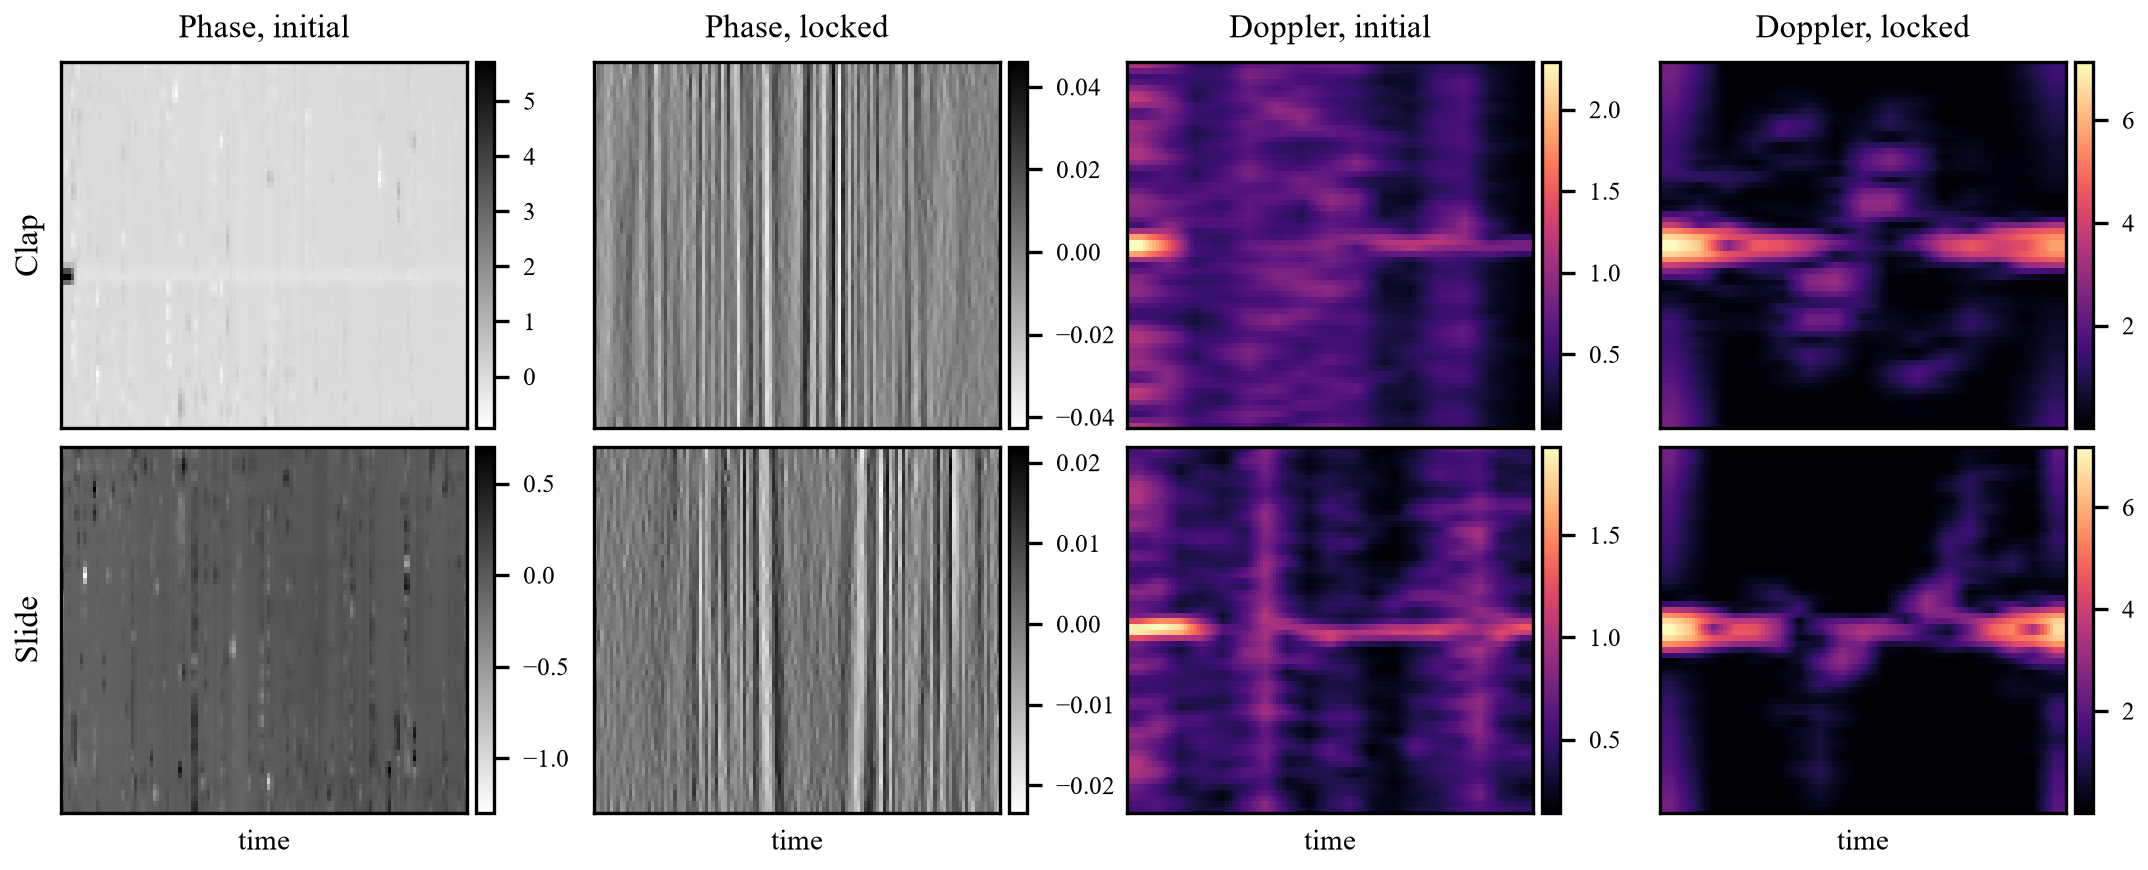
\includegraphics[width=0.9\textwidth]{figures/maps_clap_slide.png}
\caption{Phase and Doppler maps of one clap and one slide trial (user 5, training partition of the preprocessing study) under the initial pipeline (Hampel on antennas, unwrapped phase, mean-removed Doppler) and the selected pipeline. Doppler rows span $-60$ to $+60$\,Hz, with 0\,Hz in the middle.}
\label{fig:maps}
\end{figure*}

\subsection{Main results}
Table~\ref{tab:main} reports all configurations, and Fig.~\ref{fig:bars} shows target macro-F1 per task. On unseen orientations, accuracy ranges from \CzeroAcc\% to \BtwoAcc\% and macro-F1 from \CzeroFone\% to \BtwoFone\%. The matched baseline C1 reaches \ConeAcc\% accuracy and the proposed C5 \CfiveAcc\%. The paired difference of \DFiveOneAcc{} points has an interval from \DFiveOneAccLo{} to \DFiveOneAccHi, so C5 is not more accurate than C1. Its clap/slide pair error is lower, \CfiveCS\% against \ConeCS\% (\DFiveOneCS{} points, interval \DFiveOneCSLo{} to \DFiveOneCSHi), and its worst-class F1 is higher (\CfiveWorst\% against \ConeWorst\%).

\begin{table*}[t]
\centering
\caption{Results on the unseen target orientation and the in-domain test set, mean $\pm$ SD over three seeds of the three-task mean (\%). Gap: in-domain minus target macro-F1 in points.}
\label{tab:main}
\footnotesize
\begin{tabular}{@{}lcccccc@{}}
\toprule
Configuration & Target acc. & Target macro-F1 & Worst-class F1 & Clap/slide error & In-domain macro-F1 & Gap \\
\midrule
C0 & 59.16 $\pm$ 0.66 & 56.41 $\pm$ 0.89 & 22.48 $\pm$ 2.35 & 9.34 $\pm$ 0.61 & 73.04 $\pm$ 0.11 & 16.63 $\pm$ 0.78 \\
C1 (matched) & 61.54 $\pm$ 1.47 & 59.35 $\pm$ 2.11 & 31.81 $\pm$ 5.05 & 8.97 $\pm$ 2.38 & 79.85 $\pm$ 1.83 & 20.51 $\pm$ 0.93 \\
C2 & 61.46 $\pm$ 0.20 & 59.21 $\pm$ 0.24 & 29.16 $\pm$ 1.90 & 7.78 $\pm$ 1.11 & 81.01 $\pm$ 1.27 & 21.80 $\pm$ 1.19 \\
C3 & 60.73 $\pm$ 1.78 & 58.63 $\pm$ 2.01 & 33.18 $\pm$ 4.05 & 9.09 $\pm$ 0.82 & 79.15 $\pm$ 1.79 & 20.52 $\pm$ 1.73 \\
C4 & 60.57 $\pm$ 0.36 & 58.57 $\pm$ 0.42 & 34.22 $\pm$ 4.87 & 9.83 $\pm$ 2.21 & 80.38 $\pm$ 0.63 & 21.82 $\pm$ 0.24 \\
C5 (proposed) & 60.42 $\pm$ 0.68 & 58.62 $\pm$ 1.11 & 34.14 $\pm$ 1.59 & 7.14 $\pm$ 1.52 & 80.82 $\pm$ 2.09 & 22.20 $\pm$ 2.75 \\
\midrule
B1 & 60.38 $\pm$ 3.20 & 58.73 $\pm$ 3.34 & 35.67 $\pm$ 3.56 & 7.71 $\pm$ 1.10 & 80.87 $\pm$ 2.82 & 22.14 $\pm$ 0.73 \\
B2 & 62.59 $\pm$ 0.38 & 60.53 $\pm$ 0.83 & 35.83 $\pm$ 4.17 & 9.54 $\pm$ 2.07 & 83.90 $\pm$ 0.94 & 23.37 $\pm$ 1.08 \\
B3 & 60.98 $\pm$ 1.78 & 59.32 $\pm$ 1.87 & 38.36 $\pm$ 3.53 & 8.99 $\pm$ 0.69 & 80.99 $\pm$ 1.59 & 21.67 $\pm$ 1.41 \\
B4 & 59.25 $\pm$ 1.03 & 56.87 $\pm$ 1.62 & 25.81 $\pm$ 9.03 & 8.28 $\pm$ 0.94 & 79.47 $\pm$ 2.67 & 22.61 $\pm$ 2.29 \\
\bottomrule
\end{tabular}

\end{table*}

\begin{figure*}[t]
\centering
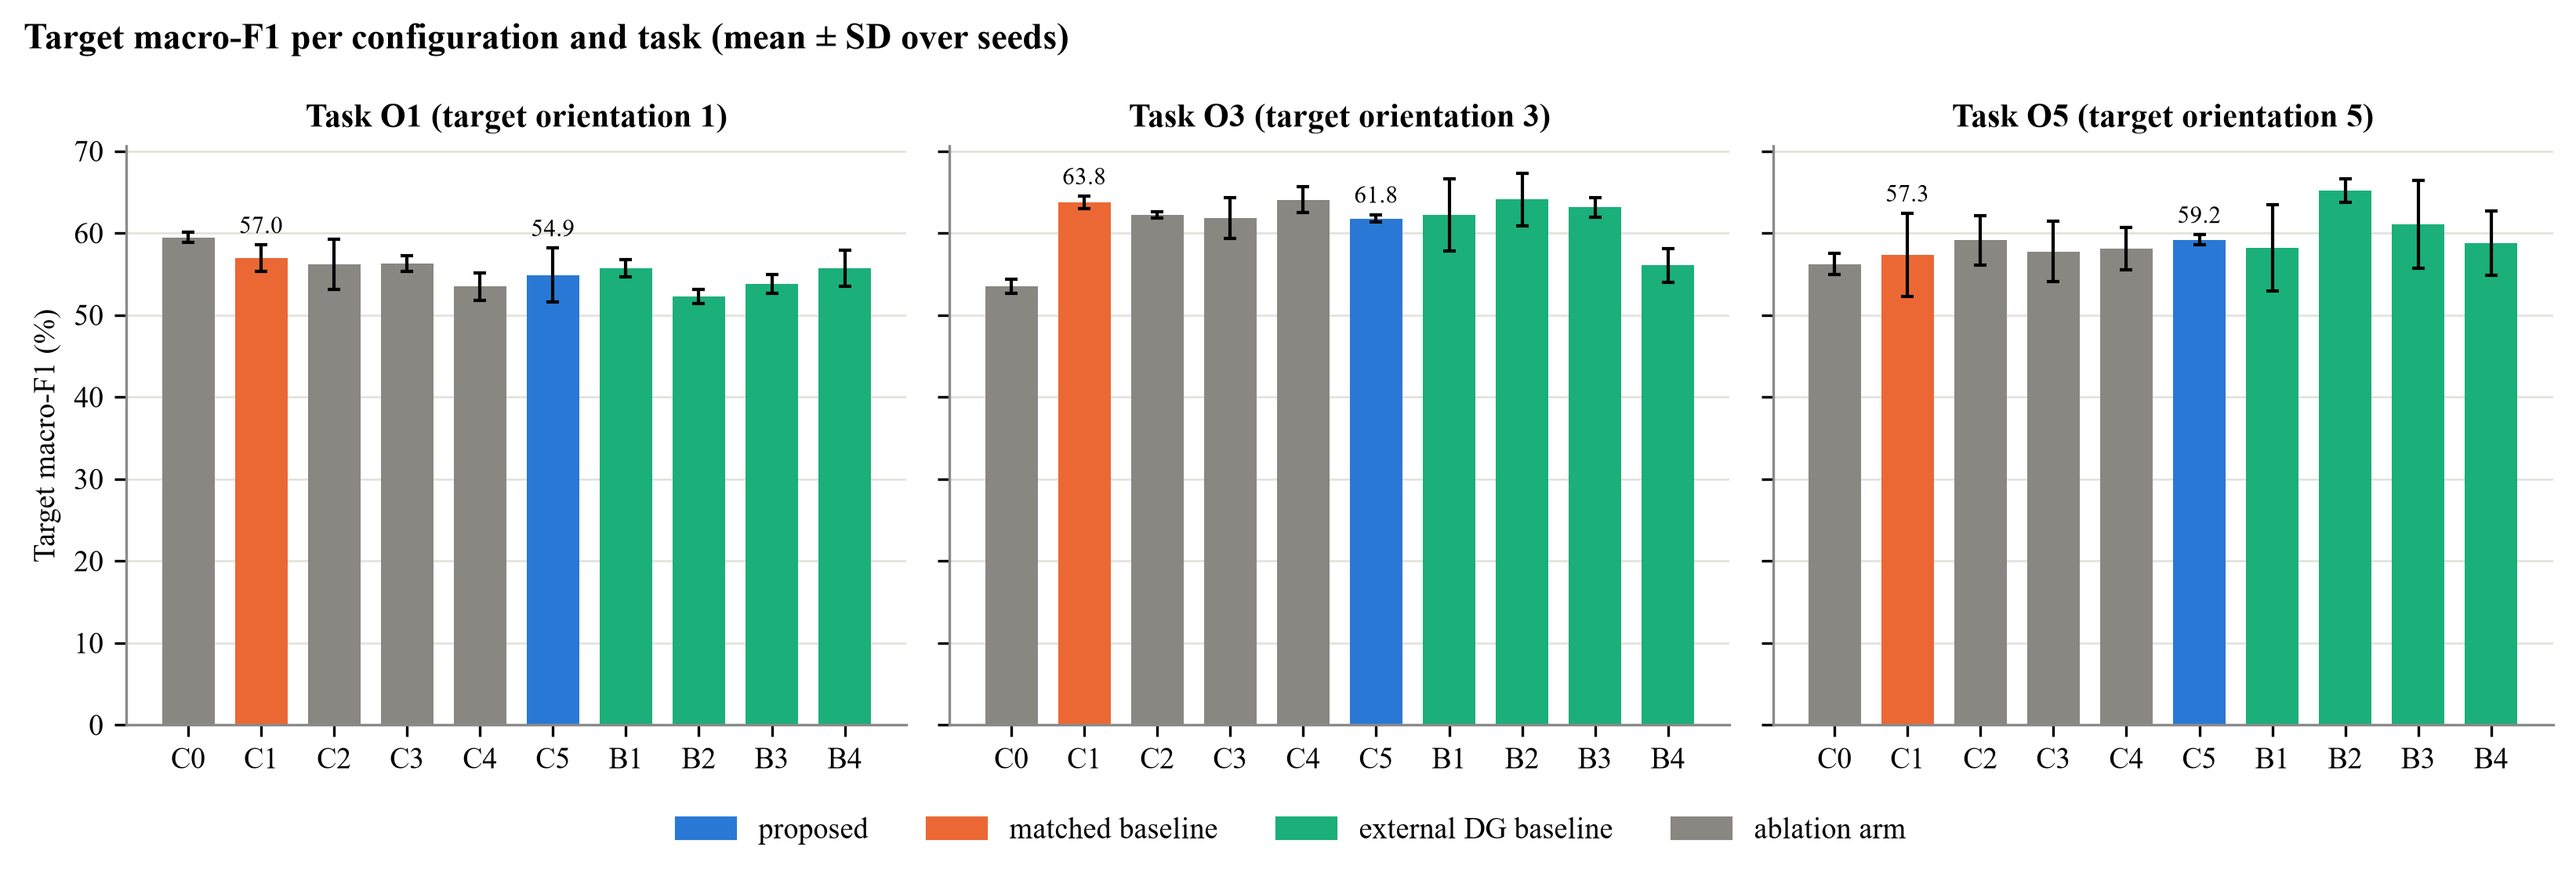
\includegraphics[width=\textwidth]{figures/F2_macro_f1_bars.png}
\caption{Target macro-F1 per configuration and task (mean $\pm$ SD over seeds). The values above C1 and C5 are their means.}
\label{fig:bars}
\end{figure*}

The external baselines behave like ERM. Selected on source validation, the best of them is B1 (ERM, \BoneSelVal\% validation macro-F1), and C5 and B1 differ by \DFiveBestAcc{} points in accuracy (interval \DFiveBestAccLo{} to \DFiveBestAccHi). Deep CORAL has the highest target accuracy (\BtwoAcc\%) but the second-lowest validation score, so it would not be chosen without looking at target data. This pattern agrees with the observation that well-tuned ERM is hard to beat in domain generalization \cite{gulrajani2021lost}.

Two results bound what any of these methods achieves. First, in-domain macro-F1 lies between 79\% and 84\% for every fused model (\ConeIDFone\% for C1, \CfiveIDFone\% for C5), well below the 97--99\% reported by multi-link and larger models; the compact single-link model does not separate the gestures fully even on orientations it has seen. Second, the generalization gap is between 20 and 24 points for every fused configuration (\ConeGap{} for C1, \CfiveGap{} for C5); the training methods move it by less than three points.

Table~\ref{tab:pertask} breaks the results down by task. The interior orientation O3 gives the highest accuracy for all four methods listed, and O5 the lowest clap/slide error. C5's lower pair error comes mostly from O1, where slide-to-clap errors fall from \ConeOoneSlideClap{} to \CfiveOoneSlideClap{} of \ConeOoneSlideN{} slide decisions (seeds pooled). The confusion matrices in Fig.~\ref{fig:cm} show where these trials go. The number of correctly recognised slides in O1 stays the same (\ConeOoneSlideCorrect{} and \CfiveOoneSlideCorrect), while slides called push\&pull rise from \ConeOoneSlidePush{} to \CfiveOoneSlidePush. Over all tasks, slide F1 falls from \ConeSlideFone\% to \CfiveSlideFone\%. The lower pair error therefore means less clap/slide mixing, not better recognition of slide.

\begin{table}[t]
\centering
\caption{Target accuracy and clap/slide error $E_{\mathrm{cs}}$ (\%) per task, mean over three seeds.}
\label{tab:pertask}
\footnotesize
\setlength{\tabcolsep}{4pt}
\begin{tabular}{@{}lcccccc@{}}
\toprule
 & \multicolumn{2}{c}{O1} & \multicolumn{2}{c}{O3} & \multicolumn{2}{c}{O5} \\
\cmidrule(lr){2-3}\cmidrule(lr){4-5}\cmidrule(lr){6-7}
 & Acc. & $E_{\mathrm{cs}}$ & Acc. & $E_{\mathrm{cs}}$ & Acc. & $E_{\mathrm{cs}}$ \\
\midrule
C1 & 60.17 & 14.38 & 64.35 & 8.67 & 60.12 & 3.85 \\
C5 & 57.99 & 9.12 & 62.67 & 7.48 & 60.59 & 4.81 \\
B1 & 58.56 & 9.94 & 63.04 & 9.19 & 59.55 & 4.00 \\
B3 & 57.05 & 11.12 & 63.90 & 11.78 & 61.97 & 4.07 \\
\bottomrule
\end{tabular}

\end{table}

\begin{figure*}[t]
\centering
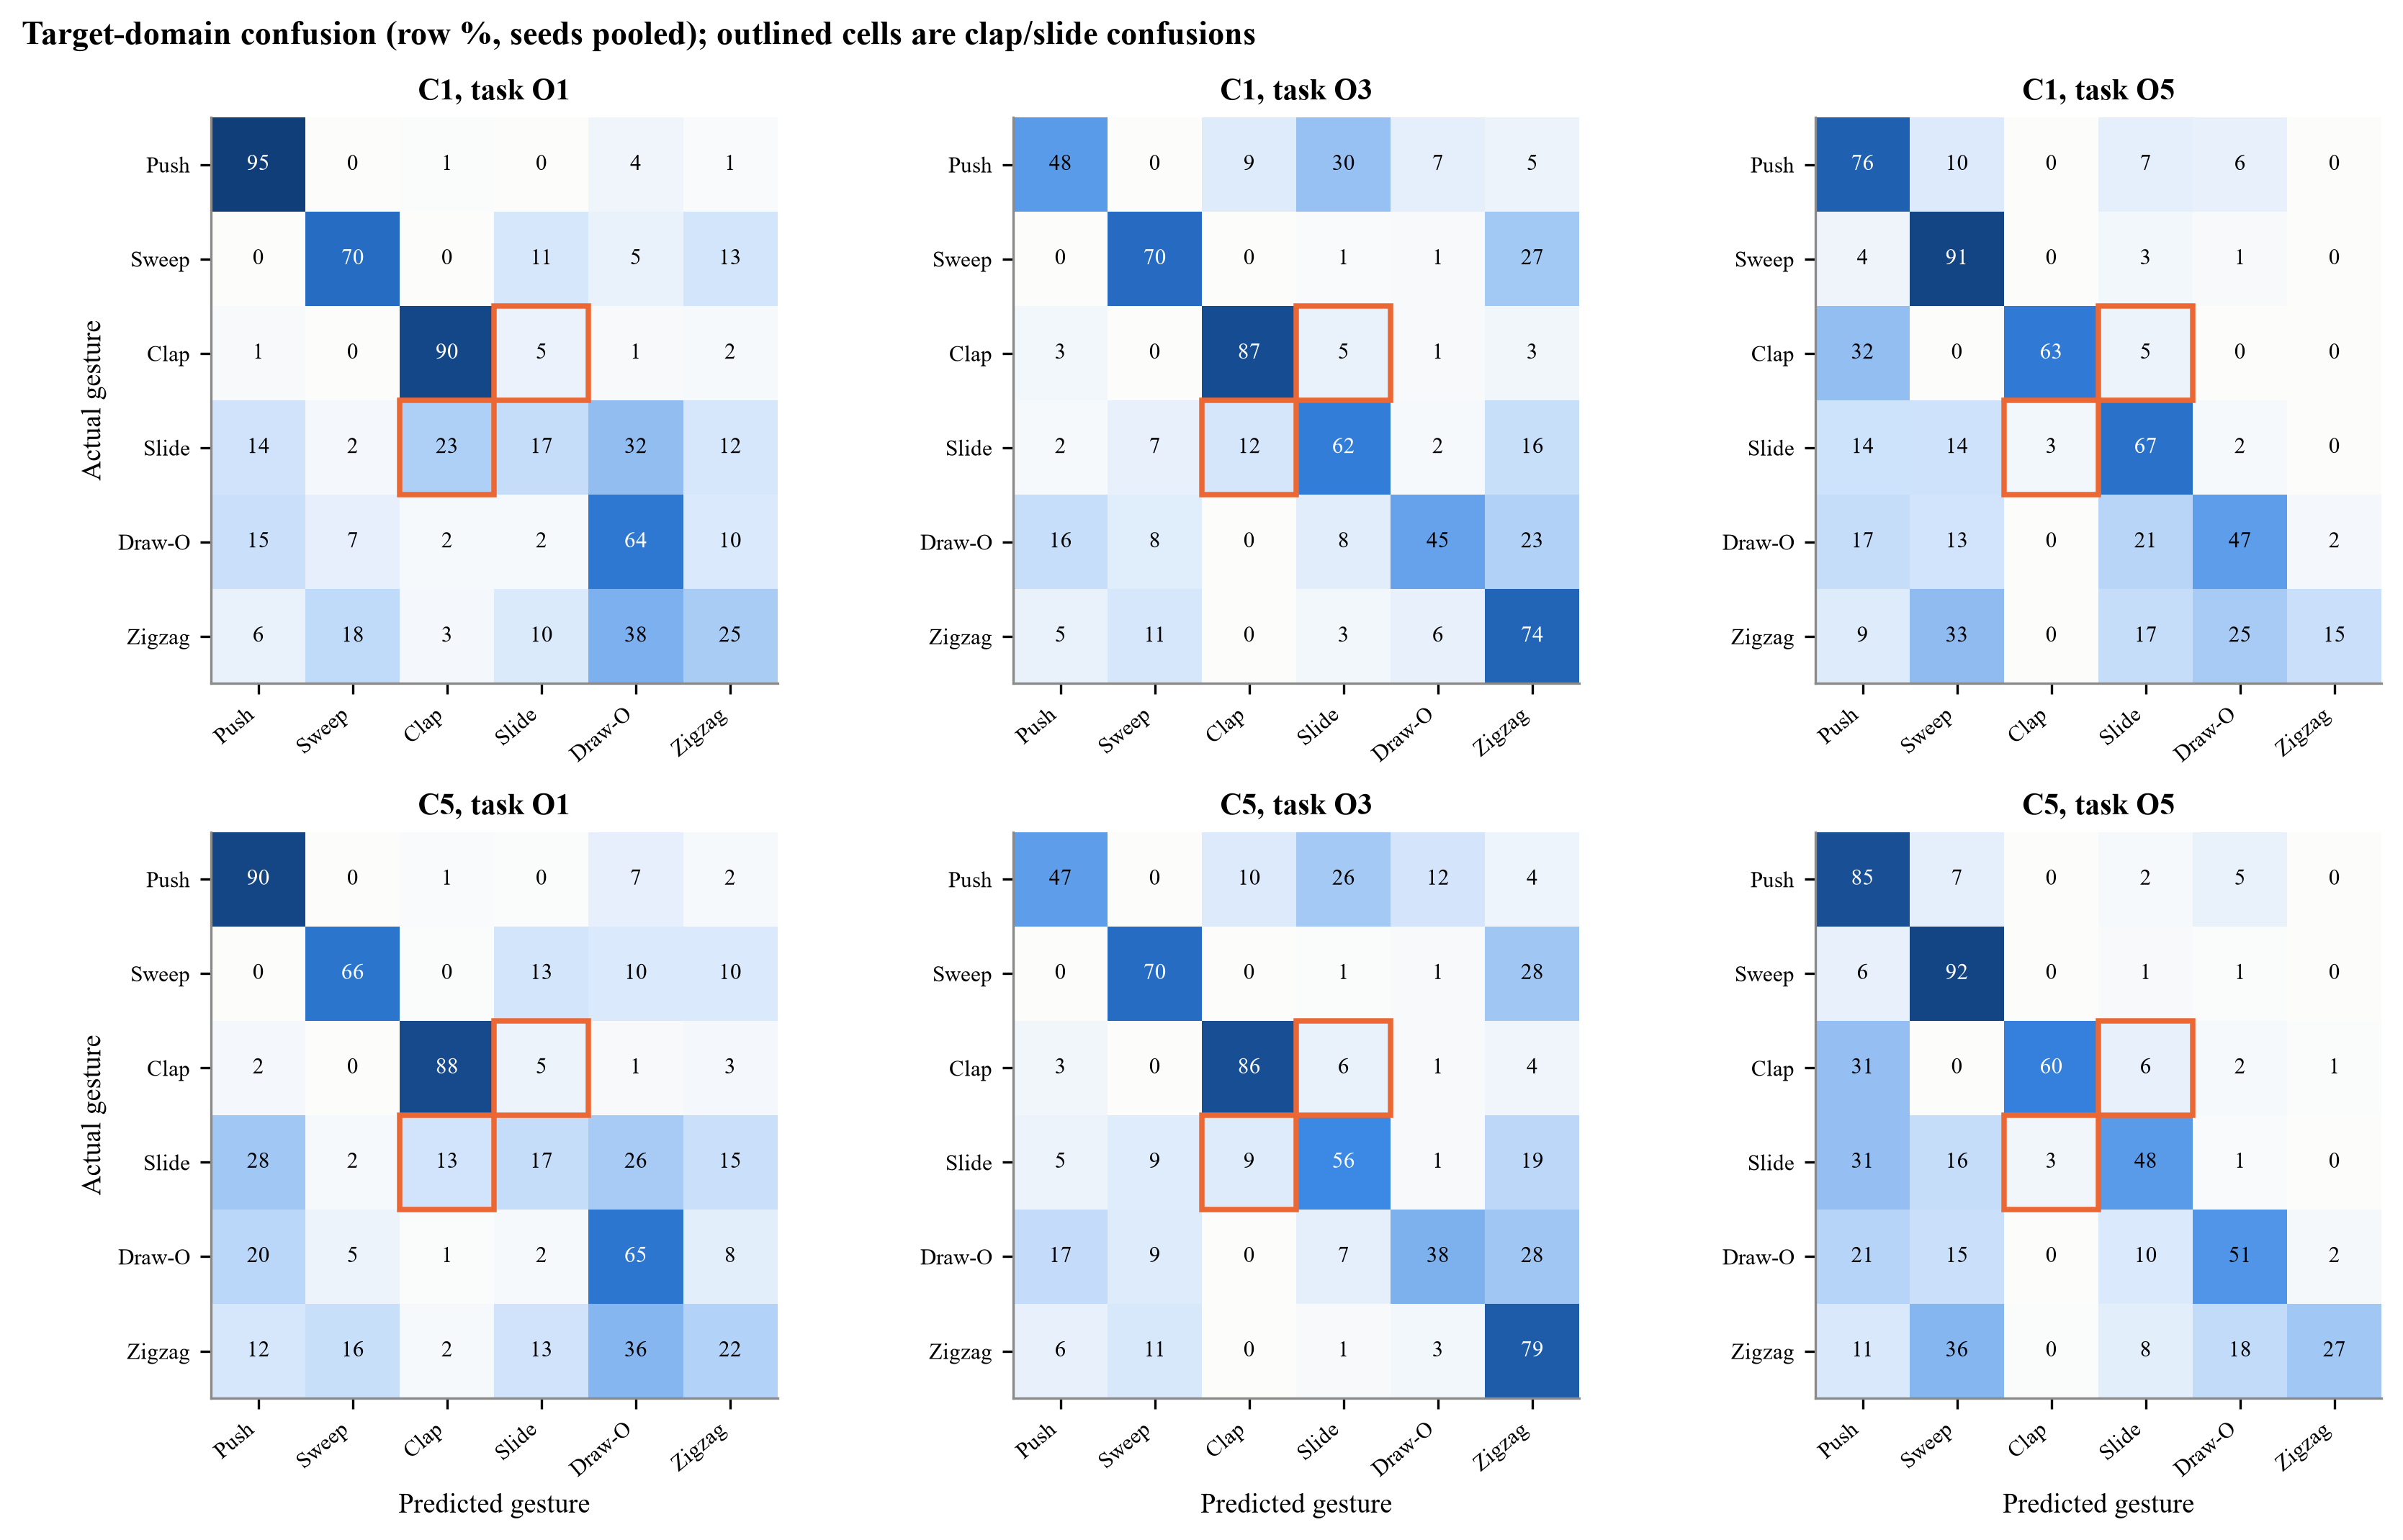
\includegraphics[width=0.85\textwidth]{figures/F4_confusion_C1_vs_C5.png}
\caption{Target confusion matrices of C1 (top) and C5 (bottom) per task, as row percentages with seeds pooled. The clap/slide cells are outlined.}
\label{fig:cm}
\end{figure*}

\textit{Cost.} Table~\ref{tab:cost} lists parameters, training time and latency. C5 adds no parameters to C1; its augmented forward pass raises training time from \ConeMinutes{} to \CfiveMinutes{} minutes per run. Inference on one trial takes a few milliseconds on the GPU; feature extraction on the CPU (\FeatMs\,ms per trial) dominates the end-to-end latency.

\begin{table}[t]
\centering
\caption{Cost per configuration on a Tesla T4. Latency: batch size one, model only.}
\label{tab:cost}
\footnotesize
\begin{tabular}{@{}lcccc@{}}
\toprule
 & Params & Train (min/run) & Median (ms) & p95 (ms) \\
\midrule
C0 & 23{,}520 & 1.25 $\pm$ 0.03 & 1.84 & 4.02 \\
C1 & 47{,}042 & 2.22 $\pm$ 0.04 & 2.93 & 6.87 \\
C5 & 47{,}042 & 2.97 $\pm$ 0.04 & 4.08 & 7.22 \\
B1 & 47{,}432 & 1.86 $\pm$ 0.10 & 2.82 & 3.86 \\
B2 & 47{,}432 & 2.16 $\pm$ 0.09 & 4.30 & 7.93 \\
B3 & 47{,}432 & 1.91 $\pm$ 0.08 & 2.84 & 5.78 \\
B4 & 47{,}432 & 1.87 $\pm$ 0.06 & 2.98 & 5.05 \\
\bottomrule
\end{tabular}

\end{table}

\section{Comparison with Base Papers}\label{sec:base}
Three studies form the base of this work. GesFi \cite{zhang2026gesfi} defines the cross-orientation protocol on Widar3.0 and its single-antenna-pair setting, WiZeCSi \cite{dai2026wizecsi} targets single-link zero-effort recognition with CSI ratios, and Koo and Park \cite{koo2026dualaxis} build a strictly single-link system for unseen users and days. Table~\ref{tab:basesum} summarises them.

\begin{table*}[t]
\centering
\caption{Summary of the base papers.}
\label{tab:basesum}
\footnotesize
\setlength{\tabcolsep}{3pt}
\begin{tabular}{@{}p{2.0cm}p{2.4cm}p{2.9cm}p{2.2cm}p{1.4cm}p{2.3cm}p{2.8cm}@{}}
\toprule
Paper & Problem & Method & Dataset & Metrics & Reported results & Key limitation \\
\midrule
Zhang et al., 2026 (GesFi) \cite{zhang2026gesfi} & domain generalization when physical domain labels misrepresent CSI shifts & latent-domain mining and adversarial alignment, ImageNet-pretrained ResNet18 & Widar3.0, ARIL, XRF55, own data & accuracy & 96.45\% CO (6 pairs), 86.66\% CO (1 pair) & trains on four orientations; no validation domain described; single runs \\
Dai and Khorov, 2026 (WiZeCSi) \cite{dai2026wizecsi} & zero-effort cross-domain recognition with few links & multi-ratio augmentation, link mixing, AlexNet-style CNN & Widar3.0 (six users), SignFi & accuracy & 98.32\% in-domain, 96.57\% CO with one test link & trains on all six receivers; 88.39\% in-domain without them \\
Koo and Park, 2026 \cite{koo2026dualaxis} & single-link finger-location sensing across users and days & dual-axis Transformer, graph network over multi-domain segments, centre loss \cite{wen2016center} & own ESP8266 data, four classes & accuracy, F1, precision & 99.31\% in-domain, 54.43\% cross-user, 56.61\% cross-day & large in-domain to cross-domain gap; different task \\
\bottomrule
\end{tabular}
\end{table*}

\textit{Quantitative comparison.} Table~\ref{tab:basequant} places the reported numbers, marked with an asterisk, next to the results of this study. No base method was re-implemented. The Widar3.0 numbers refer to the same room, gestures and receiver hardware, but not to the same protocol: both base papers train on four orientations and test on each of the five, whereas this study trains on three, reserves one for validation and tests on orientations 1, 3 and 5.

\begin{table}[t]
\centering
\caption{Accuracy (\%) of the base papers and of this work. $^{*}$Value reported in the cited paper, not reproduced.}
\label{tab:basequant}
\footnotesize
\setlength{\tabcolsep}{3pt}
\begin{tabular}{@{}p{3.6cm}cc@{}}
\toprule
Method and setting & In-domain & Cross-orient. \\
\midrule
GesFi, 6 pairs \cite{zhang2026gesfi} & -- & \RepGesFiSixCO$^{*}$ \\
GesFi, 1 pair \cite{zhang2026gesfi} & \RepGesFiOneID$^{*}$ & \RepGesFiOneCO$^{*}$ \\
GesFi, trained on 3 orientations \cite{zhang2026gesfi} & -- & \RepGesFiThreeOri$^{*}$ \\
WiZeCSi, 1 test link \cite{dai2026wizecsi} & \RepWiZeOneID$^{*}$ & \RepWiZeOneCO$^{*}$ \\
WiZeCSi, 1 link, no multi-ratio or link mixing \cite{dai2026wizecsi} & \RepWiZeAblID$^{*}$ & -- \\
Koo and Park, 1 link \cite{koo2026dualaxis} & \RepKooID$^{*}$ & n/a$^{c}$ \\
This work, C1 & \ConeIDAcc & \ConeAcc \\
This work, C5 & \CfiveIDAcc & \CfiveAcc \\
\bottomrule
\end{tabular}\\[2pt]
\raggedright\footnotesize $^{c}$Not evaluated; \RepKooCU\% cross-user and \RepKooCD\% cross-day on their own dataset.
\end{table}

\textit{Methodological differences.} The three studies obtain their accuracy partly from sources that this study excludes. WiZeCSi trains on CSI ratios from all six receivers and all antenna pairs before testing on one link; this study never sees any receiver other than r1. GesFi fine-tunes an ImageNet-pretrained ResNet18 on four training orientations; this study trains a \CfiveParams-parameter network from scratch on three. Instead of mining latent domains or adding links, the proposed method acts on the classifier: per-orientation class centres are pulled together by the consistency loss and prototypes weight orientations equally, which addresses the dependence of the decision rule on the orientation mix. Like Koo and Park, it builds training batches from several domains of the same class, and it uses the same phase and Doppler inputs that GesFi reports as the best pair.

\textit{Improvement analysis.} The proposed method does not improve on the base papers' accuracy. Its unseen-orientation accuracy differs from GesFi's single-pair result by \DiffGesFiOneCO{} points (\RelGesFiOneCO\% relative) and from WiZeCSi's single-link result by \DiffWiZeOneCO{} points (\RelWiZeOneCO\%), and its in-domain accuracy differs from WiZeCSi's single-link ablation by \DiffWiZeAblID{} points. The measurable gain of this study lies within its own controlled comparison: a change of \DFiveOneCS{} points (a \CSRelReduction\% relative reduction) in clap/slide pair error over the matched baseline, attributable to the augmentation curriculum (Section~\ref{sec:ablation}). No base paper reports this error, so it cannot be compared directly.

\textit{Fairness.} Three factors account for much of the accuracy difference, and none of them concerns the method. (i) Training orientations: GesFi's own study shows cross-orientation accuracy rising from \RepGesFiOneOri\% with one training orientation to \RepGesFiTwoOri\% with two and \RepGesFiThreeOri\% with three \cite{zhang2026gesfi}; this study uses three, and its targets include both edge orientations, which both base papers find hardest. (ii) Capacity and pretraining: a pretrained ResNet18 or AlexNet-style network against \CfiveParams{} parameters trained from scratch; the in-domain accuracy of about 80\% shows that this limits the model even without domain shift. (iii) Selection and reporting: this study selects checkpoints on a held-out source orientation and reports means over three seeds, while neither Widar3.0 base paper describes a validation domain. A protocol-matched comparison, with four training orientations and the base methods re-run under the same selection rule, remains to be done.

\section{Ablation Study}\label{sec:ablation}
Table~\ref{tab:ablation} and Fig.~\ref{fig:ablation} report the paired contrasts on the core mean.

\begin{table}[t]
\centering
\caption{Paired ablation contrasts on the three-task mean: difference in points (first row) and 95\% participant-cluster bootstrap interval (second row). A negative clap/slide difference is an improvement.}
\label{tab:ablation}
\footnotesize
\setlength{\tabcolsep}{4pt}
\begin{tabular}{@{}lccc@{}}
\toprule
Contrast & $\Delta$ acc. & $\Delta$ macro-F1 & $\Delta$ clap/slide \\
\midrule
C5 $-$ C1 & $-$1.13 & $-$0.73 & $-$1.83 \\
\quad full vs.\ matched & \scriptsize [$-$2.31, +0.06] & \scriptsize [$-$2.20, +0.51] & \scriptsize [$-$3.66, $-$0.39] \\
\addlinespace[2pt]
C5 $-$ C2 & $-$1.05 & $-$0.59 & $-$0.64 \\
\quad consistency & \scriptsize [$-$2.07, $-$0.21] & \scriptsize [$-$2.05, +0.52] & \scriptsize [$-$1.60, +0.27] \\
\addlinespace[2pt]
C5 $-$ C3 & $-$0.31 & $-$0.00 & $-$1.95 \\
\quad curriculum & \scriptsize [$-$1.31, +0.54] & \scriptsize [$-$1.12, +0.91] & \scriptsize [$-$3.38, $-$0.62] \\
\addlinespace[2pt]
C5 $-$ C4 & $-$0.16 & +0.05 & $-$2.69 \\
\quad schedule & \scriptsize [$-$0.89, +0.59] & \scriptsize [$-$0.81, +0.95] & \scriptsize [$-$4.25, $-$1.21] \\
\addlinespace[2pt]
C1 $-$ C0 & +2.39 & +2.94 & $-$0.37 \\
\quad Doppler$^{\dagger}$ & \scriptsize [+1.33, +3.46] & \scriptsize [+2.04, +3.92] & \scriptsize [$-$2.59, +1.73] \\
\addlinespace[2pt]
C5 $-$ B1 & +0.03 & $-$0.11 & $-$0.57 \\
\quad vs.\ ERM & \scriptsize [$-$1.30, +1.20] & \scriptsize [$-$1.40, +1.16] & \scriptsize [$-$1.68, +0.54] \\
\bottomrule
\end{tabular}
\\[2pt]
\raggedright\footnotesize $^{\dagger}$C1 has twice the parameters of C0, so this contrast changes capacity as well as the input.
\end{table}

\begin{figure}[t]
\centering
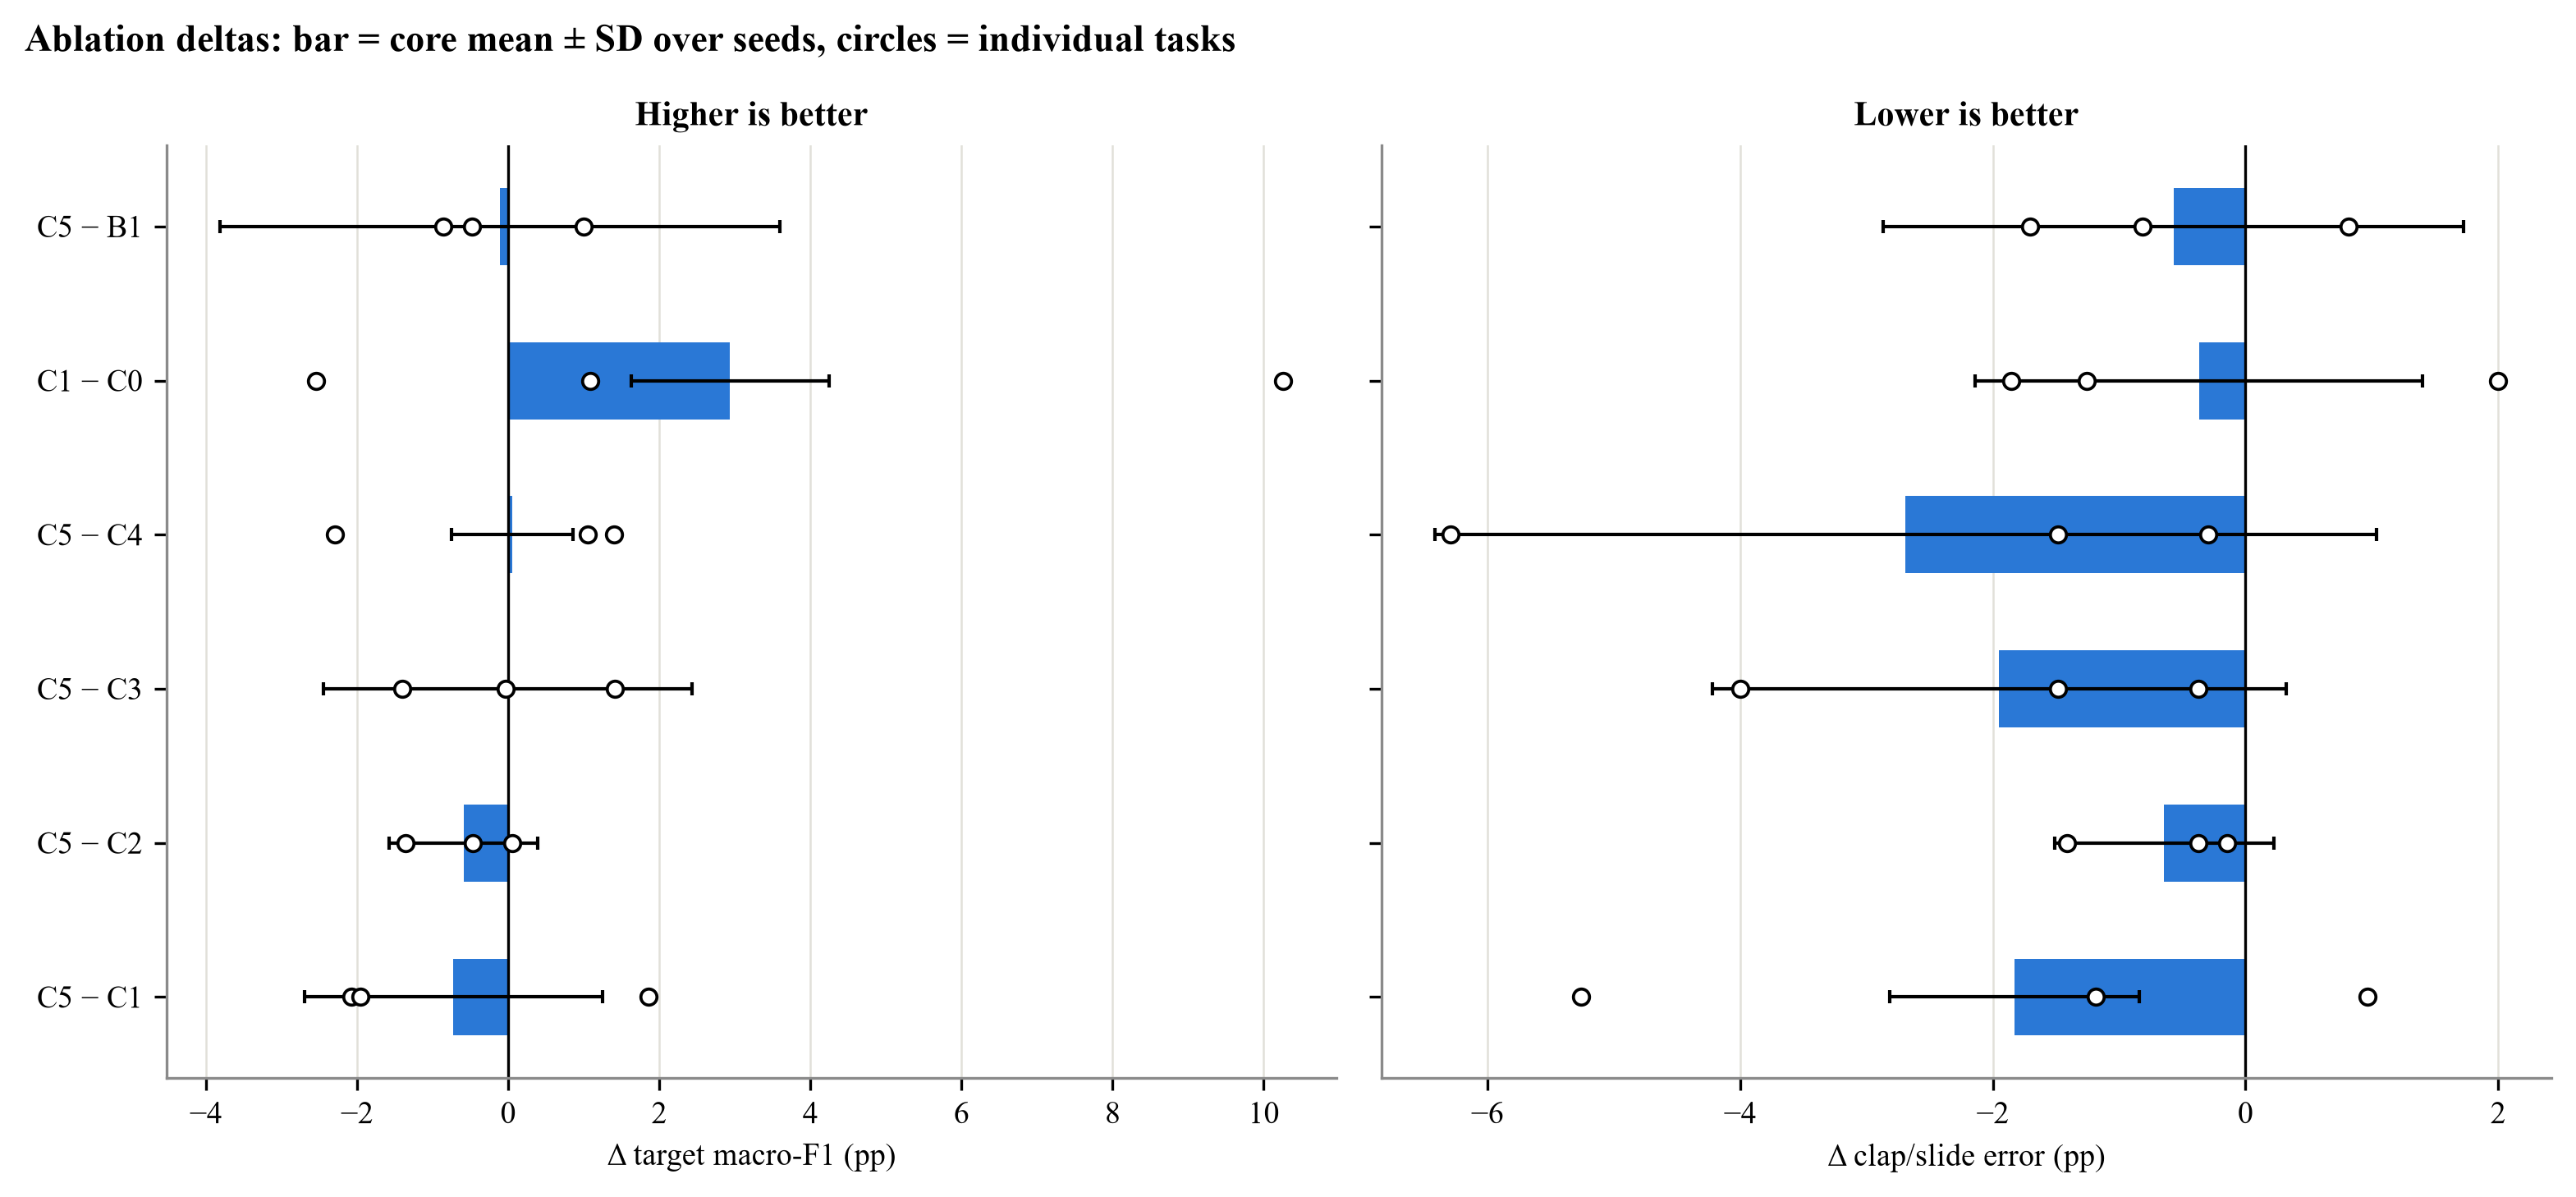
\includegraphics[width=\columnwidth]{figures/F3_ablation_deltas.png}
\caption{Ablation contrasts: bars show the three-task mean with the SD over seeds; circles show the individual tasks.}
\label{fig:ablation}
\end{figure}

\textit{Doppler branch (C1 $-$ C0).} Adding the Doppler map raises accuracy by \DOneZeroAcc{} points and macro-F1 by \DOneZeroFone{} points, with intervals that exclude zero. Because C1 also has twice as many parameters, the contrast supports, but does not isolate, the value of the Doppler input.

\textit{Class consistency (C5 $-$ C2).} Adding the consistency loss to the curriculum model changes macro-F1 by \DFiveTwoFone{} points and the pair error by \DFiveTwoCS{} points, both with intervals containing zero, and changes accuracy by \DFiveTwoAcc{} points (interval \DFiveTwoAccLo{} to \DFiveTwoAccHi). The term does not help in this setting.

\textit{Curriculum (C5 $-$ C3).} Adding the curriculum to the consistency model leaves macro-F1 unchanged and changes the pair error by \DFiveThreeCS{} points (interval \DFiveThreeCSLo{} to \DFiveThreeCSHi). This is the component behind the full method's lower pair error.

\textit{Schedule (C5 $-$ C4).} Against a fixed augmentation level after the same warm-up, the curriculum changes the pair error by \DFiveFourCS{} points (interval \DFiveFourCSLo{} to \DFiveFourCSHi) with no change in accuracy or macro-F1. Gradually increasing the augmentation helps on this error more than applying its mean strength from the start.

\textit{Consistency weight.} With seed 42, C5 reaches \LamLowFone\%, \LamMidFone\% and \LamHighFone\% target macro-F1 for $\lambda=0.05$, 0.1 and 0.3. The default $\lambda=0.1$ is not the best of the three, so the main results do not rest on a tuned weight; with one seed per value, the differences between them are not resolved.

\section{Discussion}\label{sec:discussion}
\textit{Why the method works where it does.} The curriculum perturbs the timing and Doppler content of queries while the prototypes stay clean, so the embedding must place stretched, masked and attenuated versions of a gesture near its prototype. Clap and slide differ mainly in the direction and timing of a short movement, and these perturbations seem to force the model to rely less on the cues that separate them only for some orientations. The consistency loss aims at the same goal, but in a model whose in-domain accuracy is about 80\%, pulling orientation centres together also pulls them towards a still poorly separated class mean. This agrees with GesFi's argument that aligning on physical domain labels can conflict with classification \cite{zhang2026gesfi}, as does the result that DANN with orientation labels (\BthreeAcc\%) is no better than ERM (\BoneAcc\%). The present experiments are consistent with that argument but do not test it directly.

\textit{Was the gap addressed?} The research question has two parts. The first, reducing clap/slide confusion without target data, is met: the pair error falls by \CSRelReduction\% relative to the matched baseline, and the ablation attributes the reduction to the curriculum. The second, improving single-link cross-orientation accuracy, is not met: no training method changes accuracy by more than about two points, and the stated criterion of higher accuracy and macro-F1 than C1 fails. The largest effect in the study comes from preprocessing, not from the training objective.

\textit{Practical implications.} The model has \CfiveParams{} parameters and needs one receiver with two antennas, so it can run next to the access point. In a new orientation, however, it misclassifies about four in ten gestures. For single-link deployments the evidence suggests two priorities: inputs that the model can separate in-domain, and training data that cover more orientations, rather than more complex alignment objectives.

\textit{Threats to validity.} Internal: the preprocessing was selected on orientations 2 and 4, which are never targets but serve as training or validation data in some tasks; and Deep CORAL needed a loss weight chosen on source data. External: one room, one recording session, nine users and one receiver position; the study measures orientation shift only. Construct: the pair error ignores errors into other classes, which is why per-class F1 and confusion matrices are also reported. Statistical: three seeds and nine users make the bootstrap intervals exploratory, and seeds are not independent replications of the domain shift.

\section{Conclusion and Future Work}\label{sec:conclusion}
This paper evaluated class-consistent prototype learning with an augmentation curriculum for gesture recognition from one WiFi link in unseen orientations, under a protocol that uses no target data. Preprocessing decided whether the single-link model learned at all (\GateOrig\% versus \GateLocked\% held-out accuracy). The proposed method reduced clap/slide confusion by \CSRelReduction\% relative to a matched baseline, through its curriculum, but did not raise accuracy, and four standard generalization methods stayed within about two points of ERM. The in-domain ceiling of about 80\% and the gap of about 20 points remain the main obstacles. Future work will repeat the comparison with four training orientations and the GesFi code under the same selection rule, add WiZeCSi's multi-ratio augmentation, which uses the other antenna pairs of the same receiver and so keeps the single-link constraint \cite{dai2026wizecsi}, test larger or pretrained encoders, and replace orientation labels in the consistency term with latent domains mined from the data \cite{zhang2026gesfi}.

\section*{Declarations}
\textit{Data and code availability.} Widar3.0 is publicly available from its authors \cite{zhang2022widar3}. The code, trial manifest and data splits are available at \url{https://github.com/huzaifakhallid/single-link-wifi-dg} The experiments were run with code version 04166b6 on a feature cache with SHA-256 prefix \ShaShort.

\textit{Conflict of interest.} The authors declare no conflict of interest.

\textit{Funding.} This work received no external funding.

\textit{Use of AI tools.} AI-assisted tools were used in code development and in drafting and editing the manuscript. The authors ran all experiments, verified all results and take full responsibility for the content.

\bibliographystyle{IEEEtran}
\bibliography{refs}

\end{document}
